\chapter{Von Impulsmoden zu lokalen Quantenfeldern}

Was ist ein Quantenfeld, und wie hängt es mit Teilchen zusammen? Das grundlegende mathematische Werkzeug ist der harmonische Oszillator. Ein Feld enthält viele mögliche Schwingungsmoden. Ein Feld zu quantisieren bedeutet, für jede Mode einen Quantenoszillator hinzuzufügen. Am einfachsten lässt sich die Konstruktion zunächst in einem endlichen periodischen Raum verstehen, in dem die erlaubten Moden eine diskrete Folge bilden.

\section{Periodischer Raum und erlaubte Wellenzahlen}

Man betrachte eine räumliche Koordinate \(x\) und identifiziere Punkte, die um eine Strecke \(L\) voneinander entfernt sind. Anschaulich lässt sich der Raum als Kreis mit dem Umfang \(L\) auffassen. Das ist ein nützlicher Kunstgriff, um ein endliches Volumen zu erhalten. Auf einem endlichen Intervall mit Endpunkten wird eine laufende Welle an den Enden reflektiert. Auf einem periodischen Intervall kann sie sich dagegen ohne Reflexion in beide Richtungen fortsetzen. Die Translationssymmetrie und damit die Impulserhaltung bleiben erhalten, während die Schwierigkeiten des unendlichen Volumens vorübergehend wegfallen.

Eine ebene Welle hat die Form
\begin{equation}
e^{ikx}.
\end{equation}
Nach einem Umlauf muss sie wieder ihren ursprünglichen Wert annehmen. Da die Welle bei \(x=0\) gleich \(1\) ist, verlangt die Periodizität
\begin{equation}
e^{ikL}=1.
\end{equation}
Warum erfüllt ein ganzzahliges Vielfaches von \(2\pi\) diese Bedingung? Die Euler-Formel ergibt
\begin{align}
e^{i2\pi n}
&=\cos(2\pi n)+i\sin(2\pi n)\\
&=1,
\qquad n\in\mathbb Z.
\end{align}
Der Kosinus ist nach einer beliebigen ganzen Zahl von Perioden \(1\) und der Sinus \(0\). Folglich gilt
\begin{equation}
kL=2\pi n,
\qquad
k=\frac{2\pi n}{L},
\qquad n\in\mathbb Z.
\end{equation}
Die Größe \(k\) heißt Wellenzahl. Die ganze Zahl \(n\) kennzeichnet eine erlaubte Wellenzahl; sie zählt noch keine Teilchen.

Dieselbe Bedingung lässt sich auch mithilfe der Wellenlänge ausdrücken. Eine Wellenlänge ist die Strecke, über die sich die Phase um einen vollständigen Zyklus ändert. Daher gilt
\begin{equation}
k\lambda=2\pi,
\qquad
k=\frac{2\pi}{\lambda}.
\end{equation}
Eine große Wellenlänge entspricht einer kleinen Wellenzahl, eine kleine Wellenlänge einer großen Wellenzahl. Die Periodizitätsbedingung besagt, dass eine ganzzahlige Anzahl von Wellenlängen auf den Kreisumfang passt.

Für eine quantenmechanische Welle ist der Impuls
\begin{equation}
p=\frac{h}{\lambda}
=\frac{2\pi\hbar}{\lambda}
=\hbar k.
\end{equation}
Somit unterscheiden sich \(k\) und \(p\) nur um den Faktor \(\hbar\). Positive und negative \(k\) beschreiben Wellen, die sich in entgegengesetzte Richtungen ausbreiten, und Teilchen mit entgegengesetzt gerichtetem Impuls. In Einheiten mit \(\hbar=1\) wird \(k\) üblicherweise ohne weitere Unterscheidung als Impuls bezeichnet.

Zu jeder erlaubten \(k\) kann es in dieser Mode eine bestimmte Anzahl von Quanten geben. Damit kommt eine zweite ganze Zahl ins Spiel:
\begin{equation}
n(k)=\text{number of quanta with wave number }k.
\end{equation}
Sie heißt Besetzungszahl. Die ganze Zahl in \(k=2\pi n/L\) kennzeichnet die Mode; \(n(k)\) gibt an, wie viele Teilchen diese Mode besetzen. Für negative wie für positive \(k\) müssen Besetzungszahlen angegeben werden.

\begin{classroomqa}
\lecturetimestamp{00:11:58}
\audiencequestion{Ist \(k\) selbst eine ganze Zahl?}
\lecturerresponse{Nein. Die Wellenzahl ist ein ganzzahliges Vielfaches von \(2\pi/L\): \(k=2\pi n/L\). Die ganze Zahl \(n\) in dieser Formel kennzeichnet den erlaubten Impuls und ist von der Besetzungszahl \(n(k)\) verschieden, die die Quanten in der Mode zählt.}
\end{classroomqa}

\section{Zustände mit gegebener Besetzungszahl und Modenoperatoren}

Ein Quantenzustand ist ein Vektor, also ein lineares Element. Zustandsvektoren lassen sich addieren und mit Zahlen multiplizieren; Operatoren wirken auf sie und erzeugen andere Zustandsvektoren. Beobachtbare reelle Größen werden durch hermitesche Operatoren dargestellt. Diese elementaren Tatsachen sind hier wichtig, denn sowohl der Vielteilchenzustand als auch das Feld werden aus Linearkombinationen und Operatoren aufgebaut.

Sei
\begin{equation}
k_j=\frac{2\pi j}{L},
\qquad j\in\mathbb Z.
\end{equation}
Eine praktische Kennzeichnung eines Vielteilchenzustands ist die vollständige Folge seiner Besetzungszahlen. Mit der Kurzschreibweise \(n_j\equiv n(k_j)\) für die angegebenen Einträge schreiben wir
\begin{equation}
\big|\{n(k_j)\}\big\rangle
=
\big|\ldots,n_{-2},n_{-1},n_0,n_1,n_2,\ldots\big\rangle.
\end{equation}
Der Eintrag \(n(k_1)\) gibt die Teilchenzahl in der ersten Mode mit positivem Impuls an, \(n(k_2)\) die Zahl in der zweiten und so weiter. Die Folge setzt sich in beide Richtungen unbegrenzt fort.

\begin{figure}[t]
\centering
\includegraphics[width=0.72\textwidth]{lecture_03_figure_02.png}
\caption{Besetzungszahl \(n(k)\) für eine erlaubte Impuls-Mode.}
\lectureframe{00:15:04}
\end{figure}

Jede Impuls-Mode ist ein harmonischer Oszillator. Sie besitzt daher einen Erzeugungs- und einen Vernichtungsoperator. Die zunächst als \(a^{+}(k)\) und \(a^{-}(k)\) notierte Schreibweise wird hier zu \(a^\dagger(k)\) und \(a(k)\). Ihre Wirkung ist
\begin{align}
a^\dagger(k)\big|\ldots,n(k),\ldots\big\rangle
&=
\sqrt{n(k)+1}\notag\\
&\quad{}\times
\big|\ldots,n(k)+1,\ldots\big\rangle,
\\
a(k)\big|\ldots,n(k),\ldots\big\rangle
&=
\sqrt{n(k)}\,
\big|\ldots,n(k)-1,\ldots\big\rangle.
\end{align}
Der Operator \(a^\dagger(k)\) geht zum Platz der Mode \(k\), erhöht deren Besetzung um eins und multipliziert den Zustand mit \(\sqrt{n(k)+1}\). Der Operator \(a(k)\) verringert die Besetzung desselben Platzes und liefert den Faktor \(\sqrt{n(k)}\). Für jede erlaubte Wellenzahl gibt es ein solches Operatorenpaar.

\begin{figure}[t]
\centering
\includegraphics[width=0.58\textwidth]{lecture_03_figure_03.png}
\caption{Erzeugungs- und Vernichtungsoperatoren zur Impuls-Mode \(k\).}
\lectureframe{00:17:14}
\end{figure}

\section{Fourier-Koeffizienten werden zu Operatoren}

Der Zusammenhang zwischen diesen Oszillatoroperatoren und einem Feld beginnt mit einer gewöhnlichen klassischen Fourier-Reihe. Ein komplexes klassisches Feld auf dem periodischen Intervall lässt sich schreiben als
\begin{align}
\psi(x)&=\sum_k \alpha(k)e^{ikx},\\
\psi^*(x)&=\sum_k \alpha^*(k)e^{-ikx},
\end{align}
wobei jede Summe über die erlaubten Werte \(k=2\pi n/L\) läuft. Das ist gleichbedeutend mit einer Entwicklung des Feldes in Sinus- und Kosinusfunktionen.

Das komplexe Feld besitzt einen Real- und einen Imaginärteil. Bei seiner komplexen Konjugation wechselt das Vorzeichen des Imaginärteils, und \(e^{ikx}\) wird zu \(e^{-ikx}\). Sind alle Koeffizienten \(\alpha(k)\) bekannt, ist damit das klassische Feld festgelegt. \(\alpha^*(k)\) muss dann nicht zusätzlich angegeben werden, sobald \(\alpha(k)\) bekannt ist. Real- und Imaginärteil jedes Koeffizienten sind jedoch voneinander unabhängige reelle Größen. Sie lassen sich als Amplituden der zugehörigen Fourier-Komponenten messen. In diesem Sinne fasst ein komplexer Koeffizient zwei klassische Observablen zusammen.

Bei der Quantisierung werden diese klassischen Fourier-Koeffizienten durch Operatoren ersetzt. Ein gewöhnliches Gleichheitszeichen würde Objekte unterschiedlicher Art gleichsetzen; besser ist daher eine Ersetzungsregel:
\begin{equation}
\alpha(k)\rightsquigarrow a(k),
\qquad
\alpha^*(k)\rightsquigarrow a^\dagger(k).
\end{equation}
Bei einer konsistenten Wahl der Fourier-Vorzeichen werden die Quantenfelder definiert durch
\begin{align}
\Psi(x)&=\sum_k a(k)e^{ikx},\\
\Psi^\dagger(x)&=\sum_k a^\dagger(k)e^{-ikx}.
\end{align}
\editorialnote{In der mündlichen Diskussion ändert sich die Konvention für die Fourier-Vorzeichen; später wird sie infrage gestellt. Das hier verwendete konjugierte Paar entspricht der Konvention in der klarer erkennbaren Feldentwicklung und in der Rechnung mit Ortszuständen: \(\Psi\) trägt \(e^{ikx}\) und \(\Psi^\dagger\) trägt \(e^{-ikx}\). Werden alle Vorzeichen konsistent umgekehrt, beschreibt dies dieselbe Konstruktion.}

Vorläufig ist dies eine Definition: Ein Quantenfeld ist eine Fourier-Summe, deren Koeffizienten Operatoren sind. Eine umfassendere Begründung müsste zeigen, wie diese Operatoren in einem geeigneten Grenzfall die klassischen Koeffizienten reproduzieren; dafür wäre eine Dynamik erforderlich. Diese Frage wird zurückgestellt. Klar ist bereits, dass das Feld selbst ein Operator ist und dass zwischen seinen Fourier-Koeffizienten dieselben Erzeugungs- und Vernichtungsrelationen wie bei harmonischen Oszillatoren gelten.

\begin{classroomqa}
\lecturetimestamp{00:26:48}
\audiencequestion{Bedeutet die Einführung von Erzeugungs- und Vernichtungsoperatoren, dass die Dynamik zwangsläufig Teilchen erzeugt und vernichtet?}
\lecturerresponse{Nein. Die Operatoren sind mathematische Operationen, die Besetzungszahlen ändern. Ob die Naturgesetze die Teilchenzahl tatsächlich ändern, ist eine Frage der Dynamik. Lassen die dynamischen Gesetze solche Änderungen zu, bieten diese Operatoren die natürliche Sprache, um sie zu beschreiben.}
\end{classroomqa}

\section{Streuung und veränderliche Teilchenzahl}

Betrachten wir zunächst einen Prozess, bei dem sich die Teilchenzahl nicht ändert. Angenommen, anfangs ist nur ein Teilchen mit dem Impuls \(k_7\) vorhanden. In der Besetzungszahlschreibweise hat sein Zustand im siebten Eintrag eine \(1\) und sonst überall Nullen:
\begin{equation}
|k_7\rangle
=
|\ldots,0,\underset{k_7}{1},0,\ldots\rangle.
\end{equation}
Bei einem Streuprozess ändert sich sein Impuls von \(k_7\) zu \(k_9\). Der Operator, der genau diese Änderung bewirkt, ist
\begin{equation}
a^\dagger(k_9)a(k_7).
\end{equation}
Der Operator ganz rechts wirkt zuerst: Er entfernt das Teilchen aus dem Eintrag \(k_7\). Der Operator links davon erzeugt dann ein Teilchen im Eintrag \(k_9\).

\begin{classroomqa}
\lecturetimestamp{00:31:37}
\audiencequestion{Woher kommen bei diesem Prozess \(k_7\to k_9\) die Quadratwurzelfaktoren?}
\lecturerresponse{Der Vernichtungsfaktor ist \(\sqrt{n(k_7)}=\sqrt{1}=1\). Danach befindet sich das System im Zustand, in dem alle Einträge null sind. Da die Mode \(k_9\) unbesetzt ist, beträgt der Erzeugungsfaktor \(\sqrt{n(k_9)+1}=\sqrt{1}=1\). In diesem Beispiel mit einem Teilchen ändert also keiner der beiden Faktoren den Zahlenkoeffizienten.}
\end{classroomqa}

Führen wir beide Schritte aus. Die Vernichtung ergibt
\begin{align}
a(k_7)|k_7\rangle
&=
\sqrt{1}\,|\ldots,0,0,0,\ldots\rangle\\
&=|0\rangle.
\end{align}
Der Zustand, in dem alle Einträge null sind, ist das Vakuum. Er enthält keine Teilchen und ist bei dieser einfachen Ansammlung von Oszillatoren zugleich der Grundzustand. Die Erzeugung in der unbesetzten Mode \(k_9\) ergibt dann
\begin{equation}
a^\dagger(k_9)|0\rangle
=\sqrt{0+1}\,|k_9\rangle
=|k_9\rangle.
\end{equation}
Folglich gilt
\begin{equation}
a^\dagger(k_9)a(k_7)|k_7\rangle=|k_9\rangle.
\end{equation}
Eintrag für Eintrag ist das einzige \(1\) einfach von der siebten in die neunte Impuls-Mode übergegangen. Da die Besetzung nie größer als eins war, waren beide Quadratwurzelfaktoren gleich eins. Sobald eine bereits besetzte Mode beteiligt ist, werden sie wichtig.

Dieser Eins-zu-eins-Prozess ließe sich auch mit der gewöhnlichen Einteilchen-Quantenmechanik beschreiben: Ein Teilchen ändert seinen Impuls. Die Besetzungszahlschreibweise wird unverzichtbar, wenn sich die Teilchenzahl ändern kann. Zum Beispiel beschreibt
\begin{equation}
a^\dagger(k_9)a^\dagger(k_{16})a(k_7)|k_7\rangle
=|k_9,k_{16}\rangle
\end{equation}
die mathematische Änderung von einem einlaufenden Teilchen in Mode \(k_7\) zu zwei auslaufenden Teilchen, einem in \(k_9\) und einem in \(k_{16}\). Ein Target kann das einlaufende Teilchen absorbieren, die beiden auslaufenden Teilchen emittieren und den nötigen Rückstoß aufnehmen. Ein solcher Prozess lässt sich nicht in einem auf ein Teilchen beschränkten Hilbertraum darstellen, passt aber natürlich in einen Zustandsraum mit veränderlichen Besetzungszahlen. Der Operatorausdruck ist für sich genommen kein Naturgesetz; er ist die Sprache, in der sich ein Gesetz mit veränderlicher Teilchenzahl formulieren lässt.

\section{Ein Feldoperator an einem Punkt}

Was erzeugt der Ortsraumoperator \(\Psi^\dagger(x)\)? Quantenzustände bilden einen linearen Raum: Impulszustände lassen sich mit komplexen Koeffizienten addieren, um einen neuen Zustand zu bilden. Beginnen wir mit dem Vakuum. Da jede Mode unbesetzt ist, gilt
\begin{equation}
\Psi(x)|0\rangle=0.
\end{equation}
Die Null auf der rechten Seite ist der Nullvektor: Ein Vernichtungsoperator kann kein Teilchen finden, das er entfernen könnte.

Das konjugierte Feld wirkt anders:
\begin{align}
\Psi^\dagger(x)|0\rangle
&=\sum_k e^{-ikx}a^\dagger(k)|0\rangle\\
&=\sum_k e^{-ikx}|k\rangle,
\end{align}
wobei
\begin{equation}
|k\rangle=a^\dagger(k)|0\rangle
\end{equation}
der Einteilchenzustand mit dem Impuls \(\hbar k\) ist.

\begin{figure}[t]
\centering
\includegraphics[width=0.70\textwidth]{lecture_03_figure_05.png}
\caption{Der formale Ortsraumzustand \(\Psi^\dagger(x)|0\rangle\) entwickelt in Einteilchen-Impulszustände.}
\lectureframe{00:43:16}
\end{figure}

Formal ist diese Summe, bis auf eine Normierung, der verallgemeinerte Ortszustand der Einteilchen-Quantenmechanik.\footnote{Bei unendlich vielen Impulsmoden ist ein exakt lokalisierter Ortszustand nicht normierbar. Legt man stattdessen eine endliche Impulsobergrenze fest und normiert die abgeschnittene Summe, erhält man ein scharf lokalisiertes Wellenpaket mit Zentrum bei \(x\).} Impulseigenzustände ergeben mit den Koeffizienten \(e^{-ikx}\) eine Lokalisierung bei \(x\). In diesem formalen Sinn gilt
\begin{equation}
\Psi^\dagger(x)\ \text{creates a particle at position }x,
\end{equation}
während
\begin{equation}
\Psi(x)\ \text{annihilates a particle at position }x.
\end{equation}
Der Modenoperator \(a^\dagger(k)\) erzeugt ein Teilchen mit bestimmtem Impuls. Der Feldoperator \(\Psi^\dagger(x)\) erzeugt die kohärente Überlagerung erlaubter Impulszustände, die formal bei \(x\) lokalisiert ist.

In der formalen, unnormierten Summe hat jeder Koeffizient \(e^{-ikx}\) den Betrag eins. Bei einer endlichen Impulsobergrenze besitzt der normierte, abgeschnittene Zustand für alle berücksichtigten Impulse gleich große Koeffizienten; ihre Phasen ergeben ein scharf um \(x\) lokalisiertes Wellenpaket. Das ist der elementare Zusammenhang zwischen einem Quantenfeld und Teilchen.

Lässt man zunächst die Besonderheiten der speziellen Relativitätstheorie außer Acht, erzeugt \(\Psi^\dagger(x)\) in diesem Modell ein Teilchen bei \(x\). Für relativistische Felder sind Ergänzungen nötig, doch die operatorwertige Fourier-Entwicklung und die Unterscheidung zwischen Impulsmoden- und Ortsraumoperatoren bleiben grundlegend.

\begin{classroomqa}
\lecturetimestamp{00:44:59}
\audiencequestion{Ist \(x\) ein Punkt auf dem periodischen Kreis, und was geschieht, wenn der Kreis groß wird?}
\lecturerresponse{Ja. Im endlichen Modell ist \(x\) ein Punkt auf dem Kreis. Benachbarte erlaubte Wellenzahlen haben einen Abstand von \(2\pi/L\). Mit wachsendem \(L\) wird dieser Abstand kleiner, sodass es zu jedem gewünschten Impuls einen erlaubten Wert gibt, der beliebig nahe liegt. Im Grenzfall unendlichen Volumens werden Summen über \(k\) durch Integrale über \(k\) ersetzt. Es ist hilfreich, zunächst die diskreten Summen zu verstehen.}
\end{classroomqa}

\section{Lokale Teilchenreaktionen}

Sobald \(\Psi(x)\) und \(\Psi^\dagger(x)\) als Operatoren verstanden werden, die Teilchen an einem Punkt vernichten beziehungsweise erzeugen, lässt sich Lokalität direkt ausdrücken. Man stelle sich vor, ein Teilchen werde von einem scharf bei \(x\) lokalisierten Target absorbiert, während plötzlich ein auslaufendes Teilchen nahe Alpha Centauri und ein weiteres nahe Beteigeuze erscheint. Eine solche Reaktion ist nichtlokal: Die räumlich getrennten Ereignisse können nicht durch gewöhnliche Ausbreitung miteinander verbunden werden.

Man könnte die Forderung zunächst abschwächen und erlauben, dass die auslaufenden Teilchen an beliebigen Stellen in einem kleinen Gebiet um das Target emittiert werden. Die genaue lokale Idealisierung ist stärker: Wird das einlaufende Teilchen bei \(x\) absorbiert, werden die auslaufenden Teilchen genau an diesem Punkt erzeugt. Felder an verschiedenen Punkten würden stattdessen ein nichtlokales Operatorprodukt beschreiben. Eine lokale Eins-zu-zwei-Operation lautet daher
\begin{equation}
\Psi^\dagger(x)\Psi^\dagger(x)\Psi(x).
\end{equation}
Das Feld ganz rechts entfernt das einlaufende Teilchen bei \(x\); die beiden Felder links davon erzeugen dort zwei auslaufende Teilchen.\footnote{Das lokale schematische Eins-zu-zwei-Bild folgt der bei 00:47:38--00:49:13 beschriebenen Reaktion.}

\begin{figure}[t]
\centering
\begin{tikzpicture}[scale=1.0]
\draw[->] (-2.2,0) -- (0,0);
\fill (0,0) circle (2.2pt);
\draw[->] (0,0) -- (2.0,1.1);
\draw[->] (0,0) -- (2.0,-1.1);
\node at (-1.25,0.3) {$k_{\mathrm{initial}}$};
\node[right] at (0.05,0.05) {$x$};
\node at (1.48,1.34) {$\ell$};
\node at (1.48,-1.34) {$m$};
\end{tikzpicture}
\caption{Ein einlaufendes Teilchen wird bei \(x\) absorbiert, und zwei auslaufende Teilchen werden am selben Punkt erzeugt.}
\end{figure}

Der einlaufende Zustand enthalte ein Teilchen mit der bestimmten Wellenzahl \(k_{\mathrm{initial}}\). Um die Impulse der auslaufenden Teilchen zu bestimmen, setzen wir die Impulsraum-Entwicklungen der lokalen Felder ein. Dabei muss zwischen einem festen Impulsindex und einem gebundenen Summationsindex unterschieden werden. Wir schreiben
\begin{align}
\Psi(x)&=\sum_q a(q)e^{iqx},\\
\Psi^\dagger(x)&=\sum_\ell a^\dagger(\ell)e^{-i\ell x}.
\end{align}
Über den Index \(q\) wird summiert, während \(k_{\mathrm{initial}}\) die konkret besetzte einlaufende Mode kennzeichnet. Auch für die beiden Kopien von \(\Psi^\dagger(x)\) sind unabhängige gebundene Indizes nötig, etwa \(\ell\) und \(m\). Würde man denselben Index wiederverwenden, wären die beiden unabhängigen Summen fälschlich miteinander verknüpft. Hier sind \(\ell\) und \(m\) Wellenzahlen; \(m\) bezeichnet keine Masse.

Anschaulich könnte ein Photon ein bei \(x\) lokalisiertes Atom treffen, woraufhin zwei Photonen diesen Punkt verlassen. Das hier verwendete einfache Feld eignet sich besser für nichtrelativistische Teilchen als für ein vollständig relativistisches Photonfeld. Die Rede von Photonen veranschaulicht daher nur die Buchführung der Operatoren.

Das Vernichtungsfeld wirkt zuerst:
\begin{align}
\Psi(x)|k_{\mathrm{initial}}\rangle
&=\sum_q e^{iqx}a(q)a^\dagger(k_{\mathrm{initial}})|0\rangle.
\end{align}
Alle Terme verschwinden bis auf denjenigen mit \(q=k_{\mathrm{initial}}\). Ein Vernichtungsoperator muss ein Teilchen in seiner eigenen Mode vorfinden. Daher gilt
\begin{equation}
\Psi(x)|k_{\mathrm{initial}}\rangle
=e^{ik_{\mathrm{initial}}x}|0\rangle.
\end{equation}
Die beiden Erzeugungsfelder ergeben anschließend
\begin{align}
&\Psi^\dagger(x)\Psi^\dagger(x)\Psi(x)
|k_{\mathrm{initial}}\rangle
\\
&\quad=
e^{ik_{\mathrm{initial}}x}
\sum_{\ell,m}
e^{-i\ell x}e^{-imx}
a^\dagger(\ell)a^\dagger(m)|0\rangle
\\
&\quad=
\sum_{\ell,m}
e^{i(k_{\mathrm{initial}}-\ell-m)x}
a^\dagger(\ell)a^\dagger(m)|0\rangle.
\end{align}
Für verschiedene \(\ell\) und \(m\) kann der Operatorzustand als \(|\ell,m\rangle\) bezeichnet werden: Eine der beiden Moden ist jeweils mit einem Teilchen besetzt. Das Endergebnis ist eine Summe über alle solchen Zweiteilchen-Impulskonfigurationen mit einer Phase, die von den ein- und auslaufenden Impulsen abhängt.

\begin{classroomqa}
\lecturetimestamp{01:00:36}
\audiencequestion{Kommutieren die beiden Erzeugungsoperatoren?}
\lecturerresponse{Ja. Alle Erzeugungsoperatoren kommutieren miteinander, ebenso alle Vernichtungsoperatoren. Ein Erzeugungs- und ein Vernichtungsoperator kommutieren, wenn sie sich auf verschiedene Moden beziehen; für dieselbe Mode ist ihr Kommutator ungleich null.}
\end{classroomqa}

\begin{classroomqa}
\lecturetimestamp{01:01:34}
\audiencequestion{Müssen die beiden auslaufenden Impulse die Impulserhaltung erfüllen?}
\lecturerresponse{Die dargestellten Teilchen müssen für sich genommen den Impuls nicht erhalten, denn Atom oder Target können einen Rückstoß erfahren. Die Differenz \(k_{\mathrm{initial}}-\ell-m\) ist der auf das Target übertragene Impuls. Erhalten bleibt der Gesamtimpuls einschließlich des Targets.}
\end{classroomqa}

Da der Koeffizient \(e^{i(k_{\mathrm{initial}}-\ell-m)x}\) eine reine Phase ist, hat er den Betrag eins. Zunächst scheint das auf gleiche Wahrscheinlichkeitsgewichte für alle Paare \((\ell,m)\) hinzudeuten. Wenn die beiden Indizes übereinstimmen, gilt jedoch eine wichtige Einschränkung.

Falls \(\ell=m\) gilt, setzt der erste Erzeugungsoperator ein Teilchen in die Mode \(m\), und der zweite wirkt dann auf eine bereits einmal besetzte Mode:
\begin{align}
a^\dagger(m)a^\dagger(m)|0\rangle
&=a^\dagger(m)|1_m\rangle\\
&=\sqrt{2}\,|2_m\rangle.
\end{align}
Die doppelte Erzeugung in einer Mode hat somit die zusätzliche Amplitude \(\sqrt{2}\). Beim Quadrieren der Amplitude ergibt sich in der Wahrscheinlichkeit ein Faktor \(2\).

\begin{classroomqa}
\lecturetimestamp{01:04:54}
\audiencequestion{Müssen \(\ell\) und \(m\) um eins verschieden sein, weil der Erzeugungskoeffizient \(n+1\) enthält?}
\lecturerresponse{Nein. Die Symbole \(\ell\) und \(m\) kennzeichnen Impulsmoden. Das \(n\) in \(\sqrt{n+1}\) ist die Besetzungszahl derjenigen Mode, auf die der Erzeugungsoperator wirkt. Impulsindizes und Teilchenzahlen sind verschiedene ganze Zahlen.}
\end{classroomqa}

\begin{figure}[t]
\centering
\includegraphics[width=0.92\textwidth]{lecture_03_figure_06.png}
\caption{Entwicklung der lokalen Eins-zu-zwei-Teilchen-Amplitude im Impulsraum.}
\lectureframe{01:05:44}
\end{figure}

Die Teilchen in dieser Konstruktion sind identisch. Der Faktor \(\sqrt{2}\) ist daher ein bosonischer Besetzungsfaktor und kein Index, der ein erstes von einem zweiten Teilchen unterscheidet. Sein Quadrat scheint vorläufig das Ergebnis mit gleichen Impulsen doppelt so wahrscheinlich zu machen wie einen einzelnen Term mit verschiedenen Impulsen. Sobald die Terme der Doppelsumme sorgfältig gezählt werden, muss dieser Vergleich jedoch erneut geprüft werden.

\begin{classroomqa}
\lecturetimestamp{01:06:43}
\audiencequestion{Wie wählt man bei einer komplizierten Reaktion die Reihenfolge der Erzeugungs- und Vernichtungsoperatoren?}
\lecturerresponse{Ein Ausdruck, in dem alle Erzeugungsoperatoren links und alle Vernichtungsoperatoren rechts stehen, heißt normalgeordnet. In dieser Form entfernen die Operatoren ganz rechts zuerst die einlaufenden Teilchen; die verbleibenden Operatoren erzeugen anschließend die auslaufenden Teilchen.}
\end{classroomqa}

Das Umordnen eines gemischten Erzeugungs--Vernichtungs-Paars ist im Allgemeinen keine bloße Vertauschung: Dabei muss der Kommutator verwendet werden, der für dieselbe Mode einen zusätzlichen Term liefert.\footnote{Dieser Vorbehalt zum Kommutator ist eine redaktionelle Korrektur der informellen Diskussion der Normalordnung bei 01:06:43.}

\begin{classroomqa}
\lecturetimestamp{01:07:30}
\audiencequestion{Was bedeutet eine Aussage wie ``doppelt so wahrscheinlich'', wenn die Impulsamplituden alle denselben Betrag haben?}
\lecturerresponse{Man denke an den endlichen Resonator. Seine erlaubten Impulse sind diskret, sodass sich Wahrscheinlichkeiten Modus für Modus vergleichen lassen. Verglichen werden nicht die Wahrscheinlichkeiten einzelner Punkte in einem Kontinuum.}
\end{classroomqa}

Für \(\ell\ne m\) enthält die uneingeschränkte Doppelsumme beide geordneten Terme
\begin{equation}
a^\dagger(\ell)a^\dagger(m)|0\rangle
\quad\text{and}\quad
a^\dagger(m)a^\dagger(\ell)|0\rangle.
\end{equation}

\begin{classroomqa}
\lecturetimestamp{01:08:24}
\audiencequestion{Tritt für \(\ell\ne m\) derselbe Endzustand in der Doppelsumme zweimal auf, einmal als \((\ell,m)\) und einmal als \((m,\ell)\)?}
\lecturerresponse{Ja. Wenn \(\ell\ne m\) gilt, treten sowohl die Terme \((\ell,m)\) als auch \((m,\ell)\) auf. Da die Erzeugungsoperatoren kommutieren, beschreiben beide denselben physikalischen Zustand.}
\end{classroomqa}

Die beiden geordneten Terme sind gleich. Daher müssen die Zustandsnormierung und diese doppelte Zählung berücksichtigt werden, bevor sich die Kanäle quantitativ vergleichen lassen. Die verlässliche algebraische Schlussfolgerung ist enger gefasst und genügt für das Folgende: Erzeugung in einer bereits mit \(n\) identischen Bosonen besetzten Mode liefert den Faktor \(\sqrt{n+1}\).

\section{Spontane und stimulierte Emission}

Ein übersichtlicheres Beispiel isoliert den Quadratwurzelfaktor. Ein bei \(x\) lokalisiertes Objekt emittiere ein Photon. Beginnt das Photonfeld im Vakuum, ist der auslaufende Zustand
\begin{align}
\Psi^\dagger(x)|0\rangle
&=\sum_k e^{-ikx}a^\dagger(k)|0\rangle\\
&=\sum_k e^{-ikx}|k\rangle.
\end{align}
In diesem vereinfachten Modell haben alle Impulse gleich große Amplituden. Sind zunächst keine Photonen vorhanden, ist die Emission spontan.

Nehmen wir nun an, dass sich bereits ein Photon in der Mode \(\ell\) befindet. Die Wirkung desselben lokalen Erzeugungsfeldes liefert zwei Arten von Termen:
\begin{equation}
\Psi^\dagger(x)|\ell\rangle
=
\sum_{k\ne\ell}e^{-ikx}|k,\ell\rangle
+e^{-i\ell x}\sqrt{2}\,|2_\ell\rangle.
\end{equation}
Für \(k\ne\ell\) erzeugt der Operator ein Teilchen in einer unbesetzten Mode, sodass der Koeffizient \(\sqrt{0+1}=1\) ist. Für \(k=\ell\) wirkt er auf die besetzte Mode, sodass der Koeffizient \(\sqrt{1+1}=\sqrt{2}\) ist. Das ursprüngliche Photon bleibt unbeteiligt; das neue Photon wird bevorzugt in der bereits besetzten Mode emittiert.

\begin{classroomqa}
\lecturetimestamp{01:16:14}
\audiencequestion{Muss sich das bereits vorhandene Photon am selben Ort befinden, damit es die Emission stimuliert?}
\lecturerresponse{Die vereinfachte Rechnung bezieht sich auf die Besetzung derselben Impuls-Mode, nicht darauf, dass sich zwei Teilchen an einer exakt festgelegten Position befinden. Ein Teilchen kann nicht zugleich einen exakten Ort und einen exakten Impuls haben. Reale Photonen werden durch Wellenpakete beschrieben, während die Resonator-Idealisierung diskrete Moden mit bestimmtem Impuls liefert. In diesem Rahmen erfolgt die Verstärkung in die bereits besetzte Resonatormode.}
\end{classroomqa}

Enthält die Mode \(\ell\) anfangs \(n_\ell\) Photonen, dann gilt
\begin{equation}
a^\dagger(\ell)
|\ldots,n_\ell,\ldots\rangle
=
\sqrt{n_\ell+1}
\,|\ldots,n_\ell+1,\ldots\rangle.
\end{equation}
Die Wahrscheinlichkeit wird daher um den Faktor \(n_\ell+1\) erhöht. Bei einem bereits vorhandenen Photon beträgt der Faktor \(2\). Bei hundert Photonen in der Mode ist der Amplitudenfaktor \(\sqrt{101}\) und die Wahrscheinlichkeit für eine Emission in diese Mode ist \(101\)-mal so groß wie für eine unbesetzte Mode. Je mehr Quanten eine bosonische Mode bereits enthält, desto wahrscheinlicher wird das nächste Quant in diese Mode emittiert. Das ist stimulierte Emission.

Derselbe Besetzungseffekt tritt bei Streureaktionen auf. Kann eine Kollision ein Teilchen in mehreren Moden erzeugen, erhöht eine bereits vorhandene Besetzung die Produktion in den besetzten Moden. Dies ist eine allgemeine Eigenschaft der Oszillatoralgebra und keine besondere Eigenheit des Atomzerfalls.

\begin{classroomqa}
\lecturetimestamp{01:18:15}
\audiencequestion{Haben zwei neu erzeugte Teilchen im früheren Zweiteilchenprozess weiterhin ein größeres Gewicht, wenn ihre Impulse verschieden sind?}
\lecturerresponse{Ja. In der geordneten Doppelsumme kommt ein Paar mit verschiedenen Impulsen in zwei Anordnungen vor. Der Gleichmodusfaktor \(\sqrt{2}\) verringert diesen kombinatorischen Unterschied, hebt ihn für sich genommen aber nicht auf.}
\end{classroomqa}

Wie zuvor erfordert ein physikalischer Vergleich der Kanäle weiterhin eine konsistente Normierung der Zustände und Zählweise.

\begin{classroomqa}
\lecturetimestamp{01:18:30}
\audiencequestion{Bedeutet das, dass Bosonen von bereits besetzten Impulszuständen angezogen werden?}
\lecturerresponse{Nein. Es gibt keine wirkliche Kraft und keine Anziehung. Die Verstärkung ist eine statistische Folge der Teilchenidentität und der Quadratwurzelfaktoren in den bosonischen Erzeugungsoperatoren.}
\end{classroomqa}

Es ist hilfreich, die beiden Bezeichnungen auseinanderzuhalten. Sind keine Photonen vorhanden, beginnt der Koeffizient mit \(n=0\) und ergibt den Einheitsfaktor für spontane Emission. Sind bereits Photonen vorhanden, macht der Faktor \(n+1\) die Emission in ihre Mode wahrscheinlicher; das ist stimulierte Emission.

Es gibt ein klassisches Analogon. Eine bereits vorhandene elektromagnetische Welle, die an einem Atom vorbeiläuft, treibt dessen Elektronen an. Die angeregten Elektronen strahlen stärker, als sie es ohne die Welle täten, und die zusätzliche Strahlung folgt der Richtung und Wellenzahl der anregenden Welle. In der quantenmechanischen Aussage tritt an die Stelle der vorhandenen Welle die Besetzung von Photonmoden: Vorhandene Quanten stimulieren die Erzeugung weiterer Quanten in derselben Mode.

Teilchen, für die diese harmonische Oszillatoralgebra gilt, heißen Bosonen. Sie zeigen eine statistische Tendenz, sich in bereits besetzten Zuständen anzuhäufen, ziehen einander aber nicht in diese Zustände an. Teilchen gibt es in zwei statistischen Arten: Bosonen und Fermionen. Die vorliegende Konstruktion ist bosonisch; das entgegengesetzte fermionische Verhalten wird später behandelt.

\section{Bosonische Algebra und Teilchendichte}

Zu jeder Impuls-Mode gehören Erzeugungs- und Vernichtungsoperatoren. Ihre Algebra lautet
\begin{align}
[a^\dagger(k),a^\dagger(\ell)]&=0,\\
[a(k),a(\ell)]&=0,\\
[a(k),a^\dagger(\ell)]&=\delta_{k\ell}.
\end{align}
Dabei gilt
\begin{equation}
[A,B]=AB-BA,
\end{equation}
und das Kronecker-Delta ist definiert durch
\begin{equation}
\delta_{k\ell}=
\begin{cases}
1,&k=\ell,\\
0,&k\ne\ell.
\end{cases}
\end{equation}
Erzeugungsoperatoren kommutieren bei gleichen wie bei verschiedenen Impulsen miteinander, ebenso die Vernichtungsoperatoren. Ein gemischtes Paar kommutiert bei verschiedenen Impulsen; beim gleichen Impuls gilt der bekannte Kommutator des einzelnen Oszillators.

Zusammen mit der Fourier-Definition von \(\Psi(x)\) legen diese Relationen das einfachste bosonische Quantenfeld fest. Die Aufgabe des Feldes besteht darin, Teilchen Modus für Modus oder an bestimmten Orten zu erzeugen und zu vernichten.

Betrachten wir nun den Operator
\begin{equation}
\int_0^L dx\,\Psi^\dagger(x)\Psi(x).
\end{equation}
Leiten wir ihn her, statt ihm vorab einen Namen zu geben. Durch Einsetzen der Fourier-Entwicklungen erhält man
\begin{align}
\int_0^L dx\,\Psi^\dagger(x)\Psi(x)
&=
\sum_{k,\ell}a^\dagger(k)a(\ell)
\int_0^L dx\,e^{-ikx}e^{i\ell x}
\\
&=
\sum_{k,\ell}a^\dagger(k)a(\ell)
\int_0^L dx\,e^{i(\ell-k)x}.
\end{align}
Für \(k=\ell\) ist der Exponentialfaktor \(1\), und das Integral ergibt \(L\). Für \(k\ne\ell\) wird über eine ganzzahlige Anzahl von Sinus- und Kosinusperioden entlang des Kreises integriert; positive und negative Beiträge heben sich auf. Somit gilt
\begin{equation}
\int_0^L dx\,e^{i(\ell-k)x}=L\delta_{k\ell}.
\end{equation}
Die Doppelsumme vereinfacht sich zu
\begin{equation}
\int_0^L dx\,\Psi^\dagger(x)\Psi(x)
=L\sum_k a^\dagger(k)a(k).
\end{equation}
Für jede Mode ist
\begin{equation}
a^\dagger(k)a(k)=N_k
\end{equation}
der Besetzungszahloperator. Die Summe darüber zählt alle Teilchen:
\begin{equation}
N=\sum_k N_k=\sum_k a^\dagger(k)a(k).
\end{equation}
Bei der hier verwendeten Fourier-Normierung gilt
\begin{equation}
N=\frac{1}{L}\int_0^L dx\,
\Psi^\dagger(x)\Psi(x).
\end{equation}
Bei anderen Konventionen werden Faktoren wie \(1/\sqrt{L}\) in die Fourier-Entwicklung aufgenommen, sodass der explizite Faktor \(1/L\) hier entfällt. In der verwendeten Konvention lautet der lokale Teilchendichteoperator
\begin{equation}
\rho(x)=\frac{1}{L}\Psi^\dagger(x)\Psi(x),
\qquad
\int_0^L dx\,\rho(x)=N.
\end{equation}
Somit ist \(\Psi^\dagger(x)\Psi(x)\) proportional zur Teilchendichte. Ihn als Teilchenzahl an einem mathematischen Punkt zu bezeichnen, wäre irreführend; lokal ist der Begriff Dichte angemessen.

Die Gesamtteilchenzahl kann erhalten sein oder auch nicht. Wenn die Dynamik Teilchen erzeugt oder absorbiert, kann sich \(N\) mit der Zeit ändern. Ist die Teilchenzahl unter der Dynamik erhalten, dann ist \(N\) eine erhaltene Observable.

Kennt man die Kommutatoren der Modenoperatoren, lassen sich auch die Kommutatoren von \(\Psi(x)\) und \(\Psi^\dagger(x)\) berechnen. Diese Rechnung bleibt als nützliche Übung zur Anwendung der Fourier-Summen überlassen.

Diese Konstruktion beschreibt eine Spezies identischer Bosonen. Identisch bedeutet, dass alle Teilchen von derselben Art sind, auch wenn sie unterschiedliche Orte und Impulse haben können. Elektronen und Photonen würde man nicht in dasselbe Feld \(\Psi\) einsetzen. Ein Photonenfeld erfordert relativistische Erweiterungen dieses einfachen Modells. Für ein Elektronenfeld ist eine andere, fermionische Algebra erforderlich.

\begin{classroomqa}
\lecturetimestamp{01:35:43}
\audiencequestion{Ist diese Konstruktion nur eindimensional?}
\lecturerresponse{Das bisherige Beispiel hat eine räumliche Koordinate, aber nichts Wesentliches hängt davon ab. Höhere Dimensionen erhält man durch zusätzliche Koordinaten und Impulskomponenten.}
\end{classroomqa}

\editorialnote{Ein kurzer Austausch scheint hier mit Fluoreszenz und stimulierter Emission zu beginnen und wendet sich dann Transparenz und Interferenz zu. Der beschädigte Wortlaut erlaubt keine verlässliche Rekonstruktion der Frage oder ihrer Antwort.}

Beispiele sind Photonen, das Higgs-Boson und Gravitonen.\footnote{Weitere Teilchennamen in der kurzen Beispielsaufzählung sind unklar und werden nicht übernommen.}

\section{Große Besetzung und der klassische Feldgrenzfall}

Ein komplexer Feldoperator ist für sich genommen keine einzelne hermitesche Observable. Seine beiden hermiteschen Komponenten sind
\begin{equation}
\Psi_1(x)=\frac{\Psi(x)+\Psi^\dagger(x)}{2},
\quad
\Psi_2(x)=\frac{\Psi(x)-\Psi^\dagger(x)}{2i}.
\end{equation}
Sie entsprechen in der Quantentheorie dem Real- und Imaginärteil eines klassischen Feldes. Sie kommutieren nicht, daher lassen sie sich nicht beide gleichzeitig mit beliebiger Genauigkeit messen. Für das Feld entspricht dies der Unschärfe zwischen den konjugierten Variablen eines harmonischen Oszillators.

Wann kann sich das Feld also wie eine klassische Welle verhalten? Betrachten wir eine stark angeregte Impulsmode \(k\). Ihr Besetzungszahloperator ist
\begin{equation}
a^\dagger(k)a(k)=N_k.
\end{equation}
Nehmen wir an, der Zustand habe eine große mittlere Besetzung, \(\langle N_k\rangle=n_k\gg 1\). Dann liegt die verfügbare Skala für die Amplitude eines makroskopischen Oszillators in der Größenordnung von \(\sqrt{n_k}\). Die rechte Seite von
\begin{equation}
[a(k),a^\dagger(k)]=1
\end{equation}
bleibt dagegen konstant. Der Kommutator verschwindet nie, aber bei großer Besetzung können seine Auswirkungen im Vergleich zum Quadrat der Anregungsskala klein sein. Eine große Besetzung liefert die Skala, die für einen klassischen Grenzfall erforderlich ist, genügt dafür allein jedoch nicht. Der Zustand muss außerdem hinreichend phasenkohärent sein, sodass die Unsicherheiten der beiden Quadraturen im Vergleich zur makroskopischen Feldamplitude klein sind.\footnote{Damit wird die Heuristik der großen Besetzung eingeschränkt. Ein Besetzungszahl-Eigenzustand hat \(\langle a(k)\rangle=0\), keine bestimmte Phase und Quadraturfluktuationen der Größenordnung \(\sqrt{n_k}\); für sich genommen ist er keine klassische Welle.}

Bei einem elektromagnetischen Feld bedeutet eine große Besetzung, dass viele Photonen vorhanden sind. In einem hinreichend phasenkohärenten Zustand mit vielen Photonen in den relevanten Moden verhalten sich die messbaren Feldkomponenten näherungsweise wie eine gewöhnliche klassische elektromagnetische Welle. Bei nur wenigen Photonen wird die Diskretheit der Quanten sichtbar, und die klassische Wellenbeschreibung versagt. Das Quantenfeld bleibt in beiden Bereichen ein Operator; was sich ändert, ist die relative Bedeutung seiner Quantenfluktuationen.

\begin{classroomqa}
\lecturetimestamp{01:42:09}
\audiencequestion{Bezieht sich die große Besetzungszahl auf die anfängliche oder die abschließende Besetzung?}
\lecturerresponse{Wenn sich die Photonenzahl durch den Prozess nur wenig ändert, spielt das für diese Überlegung keine Rolle. Die anfängliche und die abschließende Besetzung sind beide groß, und ihre Differenz ist im Vergleich zu beiden klein.}
\end{classroomqa}

Das entgegengesetzte Extrem ist der Grundzustand, in dem jede Besetzungszahl null ist. Dieser Zustand ist stark quantenmechanisch geprägt, und seine Schreibweise muss sorgfältig vom Nullvektor unterschieden werden.

\begin{classroomqa}
\lecturetimestamp{01:42:36}
\audiencequestion{Erzeugt ein Vernichtungsoperator, der auf das Vakuum wirkt, wieder das Vakuum oder gar keinen Zustand?}
\lecturerresponse{Er erzeugt den Nullvektor, \(a(k)|0\rangle=\mathbf{0}\). Das Vakuum \(|0\rangle\) ist ein echter normierter Zustand ohne Teilchen, der \(\langle0|0\rangle=1\) erfüllt. Es ist nicht der Nullvektor. Der Nullvektor hat Norm null und stellt keinen physikalischen Zustand dar.}
\end{classroomqa}

\begin{classroomqa}
\lecturetimestamp{01:44:11}
\audiencequestion{Ist das Feld selbst eine weitere Art von Zustand?}
\lecturerresponse{Nein. In der Quantenfeldtheorie ist das Feld ein Operator. Zustände sind Vektoren, auf die die Feldoperatoren wirken.}
\end{classroomqa}

\section{Periodischer Raum in der Praxis}

Die periodische Konstruktion ist ein Rechenhilfsmittel und keine Behauptung, das Universum sei buchstäblich ein Kreis mit einem bestimmten Umfang. Eng verwandte Systeme mit diskreten Moden kommen in der Praxis durchaus vor.

\begin{classroomqa}
\lecturetimestamp{01:45:03}
\audiencequestion{Wie wird das endliche periodische Modell in der Praxis verwendet?}
\lecturerresponse{Strahlung in einem Hohlraum mit reflektierenden Wänden liefert eine vertraute diskrete Menge von Moden. Ein Teilchen, das sich auf einem geschlossenen Draht bewegt, ist ein unmittelbar periodisches Beispiel. Es ist weder nötig noch besonders nützlich, \(L\) als Größe des Universums anzusetzen.}
\end{classroomqa}

Eine Festlegung von \(L\) führt zu einem von null verschiedenen Abstand zwischen benachbarten Impulsen, aber die Anzahl der Impulse bleibt unendlich.

\begin{classroomqa}
\lecturetimestamp{01:45:39}
\audiencequestion{Begrenzt eine Festlegung der Länge \(L\) die Gesamtzahl möglicher Impulszustände?}
\lecturerresponse{Nein. Die erlaubten Werte sind \(k_j=2\pi j/L\), und \(j\) kann eine beliebige ganze Zahl sein, sodass es weiterhin unendlich viele Moden gibt. Bei endlichem \(L\) gibt es lediglich unterhalb eines gewählten Maximalimpulses endlich viele Moden. Ohne eine solche Abschneidung bleibt die Impulsquantenzahl unbeschränkt.}
\end{classroomqa}

Die Oszillatorinterpretation lässt sich auch umgekehrt betrachten. In der elementaren Oszillatormechanik beginnt man mit konjugierten Variablen und bildet daraus \(a\) und \(a^\dagger\). Hier wurden zuerst die Modenoperatoren eingeführt, daher liegt die Frage nahe, wo ihre konjugierten Variablen auftreten.

\begin{classroomqa}
\lecturetimestamp{01:46:43}
\audiencequestion{Was entspricht bei einer festen Mode den Oszillatorvariablen \(X\) und \(P\), wenn die Konstruktion mit \(a(k)\) und \(a^\dagger(k)\) beginnt?}
\lecturerresponse{Zu jeder festgelegten Impulsmode gehört ein Oszillator. Seine beiden hermiteschen Quadraturen werden aus \(a(k)\) und \(a^\dagger(k)\) gebildet, so wie die reellen und imaginären Feldkomponenten aus \(\Psi\) und \(\Psi^\dagger\) gebildet werden. Bis auf Normierung und eine mögliche Vertauschung der Bezeichnungen entsprechen sie \(X\) und \(P\).}
\end{classroomqa}

Für die feste Mode lauten die Quadraturen, wenn man von konventionsabhängigen numerischen Faktoren absieht:\footnote{Der Austausch bei 01:46:43 wechselt in grober Formulierung zwischen einer einzelnen Impulsmode und dem gesamten Feld. Die angegebene Beziehung macht die Aussage für eine feste Mode explizit: \(\Psi(x)\) und \(\Psi^\dagger(x)\) sind Fourier-Summen über alle Moden.}
\begin{equation}
X_k\propto a(k)+a^\dagger(k),
\qquad
P_k\propto \frac{a(k)-a^\dagger(k)}{i}.
\end{equation}
Die zuvor eingeführten Ortsraumkomponenten \(\Psi_1(x)\) und \(\Psi_2(x)\) sind Fourier-Überlagerungen dieser Modenquadraturen und nicht die Quadraturen einer einzelnen festen Mode. Ihre Unschärferelation ist dasselbe Hindernis, auf das man stößt, wenn man ein schwach angeregtes Quantenfeld als vollständig klassisches Objekt auffassen will.

\section{Periodischer Raum in höheren Dimensionen}

\begin{classroomqa}
\lecturetimestamp{01:48:21}
\audiencequestion{Wie wird periodischer Raum in mehr als einer Dimension dargestellt?}
\lecturerresponse{In zwei Dimensionen ist der Torus das Analogon zum Kreis. Man kann ihn als Rechteck darstellen, bei dem die linke und rechte Kante miteinander identifiziert sind und ebenso die untere und obere Kante. Es gibt zwei periodische Richtungen, daher sind beide Impulskomponenten quantisiert.}
\end{classroomqa}

Ein Torus wird oft als Donutoberfläche dargestellt, doch für Rechnungen ist ein Rechteck nützlicher. Schneidet man die Oberfläche einmal auf, lässt sie sich zu einem Zylinder aufklappen. Schneidet man den Zylinder ein weiteres Mal auf, kann man ihn flach ausbreiten. Das entstehende Rechteck trägt weiterhin zwei Identifikationen: Die linke Kante ist mit der rechten identisch, und die untere mit der oberen.\footnote{Das Rechteck, seine beiden Kantenidentifikationen, das Wiedererscheinen des Teilchens und die Aussage, dass beide Impulskomponenten quantisiert sind, ergeben sich aus 01:48:46--01:50:58. Die angegebenen Formeln für \(k_x\) und \(k_y\) ergeben sich komponentenweise aus der früheren Bedingung \(kL=2\pi n\).}

Ein Teilchen, das die rechte Kante überquert, erscheint am entsprechenden Punkt auf der linken Kante wieder. Überquert es die obere Kante, erscheint es am entsprechenden Punkt auf der unteren wieder. Ein periodisches Feld erfüllt
\begin{align}
\Psi(x+L_x,y)&=\Psi(x,y),\\
\Psi(x,y+L_y)&=\Psi(x,y).
\end{align}
Für eine ebene Welle \(e^{i(k_x x+k_y y)}\) erfordern diese Identifikationen
\begin{equation}
k_x=\frac{2\pi n_x}{L_x},
\qquad
k_y=\frac{2\pi n_y}{L_y},
\qquad
n_x,n_y\in\mathbb Z.
\end{equation}
Beide Impulskomponenten sind diskret.

\begin{figure}[t]
\centering
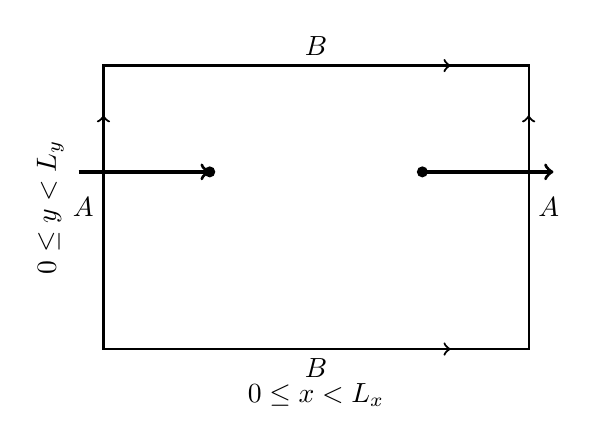
\begin{tikzpicture}[x=0.9cm,y=0.9cm]
\draw[thick] (0,0) rectangle (6,4);
\draw[->,thick] (0,0.7) -- (0,3.3);
\draw[->,thick] (6,0.7) -- (6,3.3);
\draw[->,thick] (1.1,0) -- (4.9,0);
\draw[->,thick] (1.1,4) -- (4.9,4);
\node[left] at (0,2) {$A$};
\node[right] at (6,2) {$A$};
\node[below] at (3,0) {$B$};
\node[above] at (3,4) {$B$};
\draw[->,very thick] (4.5,2.5) -- (6.35,2.5);
\draw[->,very thick] (-0.35,2.5) -- (1.5,2.5);
\fill (4.5,2.5) circle (2pt);
\fill (1.5,2.5) circle (2pt);
\node at (3,-0.65) {$0\leq x<L_x$};
\node[rotate=90] at (-0.75,2) {$0\leq y<L_y$};
\end{tikzpicture}
\caption{Ein zweidimensionaler periodischer Raum: Kanten mit gleicher Bezeichnung sind identifiziert, sodass ein Teilchen, das eine Kante überquert, am entsprechenden Punkt der gegenüberliegenden Kante wieder erscheint.}
\end{figure}

\begin{classroomqa}
\lecturetimestamp{01:50:58}
\audiencequestion{Beschreibt die periodische Konstruktion den Raum oder die Objekte im Raum?}
\lecturerresponse{Sie beschreibt den Raum. Die Objekte und Felder befinden sich in diesem Raum und erfüllen seine Identifikationen. Die Periodizität wird eingeführt, um das Problem des unendlichen Volumens zu kontrollieren; man entfernt sie, indem man das Volumen groß werden lässt und Impulssummen durch Integrale ersetzt.}
\end{classroomqa}

Das dreidimensionale Analogon ist ein Würfel, bei dem jeweils zwei gegenüberliegende Flächen identifiziert sind. Die linke und rechte Fläche sind identisch, ebenso die obere und untere sowie die vordere und hintere. Ein Teilchen, das eine Fläche überquert, erscheint durch die mit ihr identifizierte Gegenfläche wieder.\footnote{Der periodische Würfel und seine drei Paare identifizierter Flächen ergeben sich aus 01:51:27--01:52:17. Die angegebene Gleichung für \(k_i\) ergibt sich komponentenweise aus der früheren Bedingung \(kL=2\pi n\), angewandt auf die drei periodischen Richtungen.} Die drei Impulskomponenten erfüllen
\begin{equation}
k_i=\frac{2\pi n_i}{L_i},
\qquad i=x,y,z,
\end{equation}
mit einer ganzen Zahl \(n_i\) für jede Richtung. Nach derselben Regel lassen sich Tori in beliebig vielen Dimensionen definieren.

\begin{figure}[t]
\centering
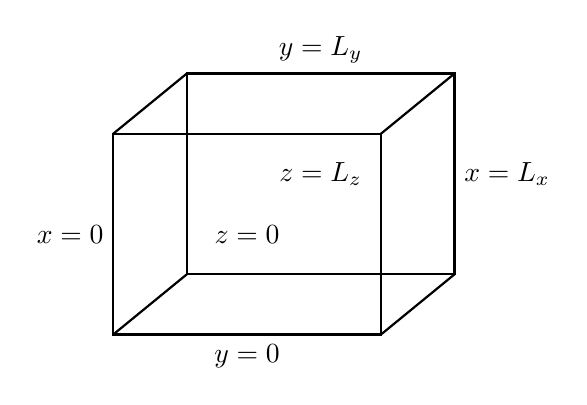
\begin{tikzpicture}[scale=0.85]
\draw[thick] (0,0) rectangle (4,3);
\draw[thick] (1.1,0.9) rectangle (5.1,3.9);
\draw[thick] (0,0) -- (1.1,0.9);
\draw[thick] (4,0) -- (5.1,0.9);
\draw[thick] (4,3) -- (5.1,3.9);
\draw[thick] (0,3) -- (1.1,3.9);
\node[left] at (0,1.5) {$x=0$};
\node[right] at (5.1,2.4) {$x=L_x$};
\node[below] at (2,0) {$y=0$};
\node[above] at (3.1,3.9) {$y=L_y$};
\node at (2,1.5) {$z=0$};
\node at (3.1,2.4) {$z=L_z$};
\end{tikzpicture}
\caption{Ein dreidimensionaler periodischer Raum als Würfel, bei dem jeweils zwei gegenüberliegende Flächen identifiziert sind.}
\end{figure}

\begin{classroomqa}
\lecturetimestamp{01:52:20}
\audiencequestion{Legt die Feldtheorie eine physikalische Gitterweite für den Raum fest?}
\lecturerresponse{Das ist eine spekulative Frage. Für die hier betrachteten Zwecke ist der Raum kontinuierlich. Die Quanten sind Teilchen und keine Zellen eines räumlichen Gitters. In der Konstruktion mit dem Kreis wird der Impuls diskret; der Ort bleibt kontinuierlich und periodisch.}
\end{classroomqa}

\editorialnote{Eine längere beschädigte Passage während des Austauschs über die Gitterweite erwähnt Planck-Skalen, enthält aber keine rekonstruierbare Aussage über eine fundamentale Diskretheit des Raums. Eine solche Aussage wird hier nicht abgeleitet.}

Die Diskretheit von \(k\) entstand ausschließlich dadurch, dass eine periodische Wellenfunktion vorgeschrieben wurde. Sie ist kein Beleg dafür, dass die Koordinate \(x\) selbst auf einem Gitter liegt. Zu fragen, ob der Raum eine fundamentale mikroskopische Struktur haben könnte, ist legitim, aber es handelt sich um eine eigenständige spekulative Frage.

\section{Fermionen und äußere Felder}

Bosonische Moden erlauben jede nichtnegative Besetzungszahl. Für Fermionen gilt das Gegenteil: Das Pauli-Ausschlussprinzip verbietet es zwei identischen Fermionen, denselben Zustand zu besetzen.

\begin{classroomqa}
\lecturetimestamp{01:55:13}
\audiencequestion{Erhält man die einfachste Fermionentheorie, indem man Kommutatoren durch Antikommutatoren ersetzt?}
\lecturerresponse{Im Wesentlichen ja. Der Kommutator ist \([A,B]=AB-BA\), der Antikommutator hingegen \(\{A,B\}=AB+BA\). Die entsprechende fermionische Erzeugungs- und Vernichtungsalgebra verwirklicht das Pauli-Ausschlussprinzip: Ein zweites identisches Fermion kann nicht in einen bereits besetzten Zustand gebracht werden. Die ausführliche Theorie folgt später.}
\end{classroomqa}

Die beiden Produkte unterscheiden sich durch ein Vorzeichen:
\begin{equation}
[A,B]=AB-BA,
\qquad
\{A,B\}=AB+BA.
\end{equation}
Der Kommutator ist unter Vertauschung antisymmetrisch, der Antikommutator dagegen symmetrisch. Verschwindet ein Antikommutator, dann gilt
\begin{equation}
\{A,B\}=0
\quad\Longrightarrow\quad
AB=-BA.
\end{equation}
Beim Vertauschen eines solchen Operatorpaars ändert sich das Vorzeichen. Das ist ungewöhnlicher als gewöhnliches Kommutieren, bei dem \([A,B]=0\) gilt und daraus \(AB=BA\) folgt. Die bosonischen Kommutatoren durch die entsprechende antikommutierende Algebra zu ersetzen, ist die mathematische Änderung, die zu Fermionen führt; ihre ausführliche Entwicklung wird auf später verschoben.

Antikommutieren kehrt das statistische Verhalten von Bosonen um. Identische Fermionen häufen sich nicht durch stimulierte Besetzung in einer Mode; die Besetzung dieser Mode verhindert, dass ein weiteres identisches Fermion hinzukommt. Da ein einzelner fermionischer Zustand höchstens ein identisches Fermion enthalten kann, erhält man keinen klassischen Feldgrenzfall, indem man beliebig viele von ihnen in diesen einen Zustand bringt.

\begin{classroomqa}
\lecturetimestamp{01:58:03}
\audiencequestion{Wie kann ein Alphateilchen ein Boson sein, wenn es aus Fermionen besteht?}
\lecturerresponse{Ein gebundenes zusammengesetztes Teilchen mit einer geraden Anzahl fermionischer Bestandteile kann bosonische Statistik aufweisen. Mehrere solcher zusammengesetzten Bosonen in denselben Gesamtzustand zu bringen, ist nicht dasselbe, wie ihre einzelnen fermionischen Bestandteile in ein und denselben identischen Einteilchenzustand zu bringen.}
\end{classroomqa}

Die zusammengesetzte Statistik betrifft das gebundene Objekt als Ganzes. Fermionische Bestandteile können sich daher zu einem Objekt verbinden, das sich wie ein Boson verhält, ohne das Ausschlussprinzip für die Bestandteile zu verletzen.

\begin{classroomqa}
\lecturetimestamp{01:58:33}
\audiencequestion{Wie werden äußere Felder einbezogen?}
\lecturerresponse{In der bisherigen Konstruktion wurde kein äußeres Hintergrundfeld berücksichtigt. Ein solches Feld kann als klassisches Feld vorgegeben oder quantenmechanisch durch einen Zustand mit einer großen Zahl von Quanten dargestellt werden.}
\end{classroomqa}

Damit beide Beschreibungen übereinstimmen, muss der Zustand mit großer Besetzung passend präpariert und phasenkohärent sein; die Teilchenzahl allein genügt nicht.\footnote{Der Austausch liefert die Skala mit vielen Quanten. Die Phasenkohärenz wird hier als zusätzliche Bedingung genannt, damit eine große Besetzung allein nicht mit einem klassischen Feld verwechselt wird.} In diesem semiklassischen Bereich stimmen ihre Wirkungen bis auf kleine Quantenabweichungen überein. Dies ist eine grundlegende Konsistenzbedingung. Das elektromagnetische Feld muss einzelne Photonen beschreiben, wenn einzelne Quanten relevant sind, und zugleich muss ein hinreichend phasenkohärenter Zustand mit vielen Photonen die vertraute Wirkung einer klassischen elektromagnetischen Welle reproduzieren.